\documentclass[logo,reportComp]{thesis}
\usepackage[cpp,pseudo]{mypackage}

\usetikzlibrary{automata,backgrounds,fit,shapes,positioning}

\tikzset{->, % makes the edges directed
>=stealth, % makes the arrow heads bold
node distance=2.5cm, % specifies the minimum distance between two nodes. Change if necessary.
every state/.style={thick, fill=gray!10}, % sets the properties for each 'state' node
}

\title{编译原理作业三}
\subtitle{}
\school{数据科学与计算机学院}
\author{陈鸿峥}
\classname{17大数据与人工智能}
\stunum{17341015}
\headercontext{编译原理作业}

% May 9 -> May 14

\begin{document}

\maketitle

\begin{question}
考虑以下DFA的状态迁移表,其中$0$,$1$为输入符号,$A\thicksim H$代表状态:
\begin{center}
\begin{tabular}{|c|c|c|}\hline
 & \textbf{0} & \textbf{1} \\\hline
\textbf{A} & B & A \\\hline
\textbf{B} & A & C \\\hline
\textbf{C} & D & B \\\hline
\textbf{D} & D & A \\\hline
\textbf{E} & D & F \\\hline
\textbf{F} & G & E \\\hline
\textbf{G} & F & G \\\hline
\textbf{H} & G & D \\\hline
\end{tabular}
\end{center}
其中$A$为初始状态,$D$为接受状态,请画出与此DFA等价的最小DFA,并在新的DFA状态中标明它对应的原DFA状态的子集.
\end{question}
\begin{answer}
由最小化状态算法,初始化划分$\Pi$为接受状态组$(D)$和非接受状态组$(ABCEFGH)$。
对于非接受状态组,输入$0$,$(CE)$会跳转至另一个组的成员,因此需要被划分,得到$\Pi_{new}=(ABFGH)(CE)(D)$。
再考虑$(ABFGH)$,输入$1$,$(BF)$会跳转至另一个组$(CE)$,$(H)$会跳转到$(D)$,因此都得被划分。
最终得到$\Pi_{final}=(AG)(BF)(H)(CE)(D)$,可画出下面的最小DFA。
\begin{center}
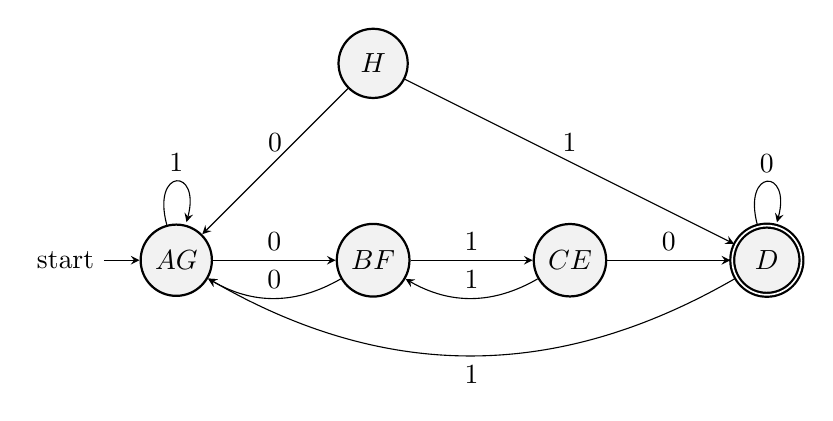
\begin{tikzpicture}
\node[state, initial] (1) {$AG$};
\node[state, right of=1] (2) {$BF$};
\node[state, right of=2] (3) {$CE$};
\node[state, accepting, right of=3] (4) {$D$};
\node[state, above of=2] (5) {$H$};
\draw (1) edge[above] node{$0$} (2)
(1) edge[loop above] node{$1$} (1)
(2) edge[bend left, above] node{$0$} (1)
(2) edge[above] node{$1$} (3)
(3) edge[bend left, above] node{$1$} (2)
(3) edge[above] node{$0$} (4)
(4) edge[loop above] node{$0$} (4)
(4) edge[bend left, below] node{$1$} (1)
(5) edge[above] node{$0$} (1)
(5) edge[above] node{$1$} (4);
\end{tikzpicture}
\end{center}
\end{answer}

\begin{question}
考虑所有含有$3$个状态(设为$p$,$q$,$r$)的DFA.
设只有$r$是接受状态. 至于哪一个状态是初始状态与本问题无关.
输入符号只有$0$和$1$. 这样的DFA总共有$729$种不同的状态迁移函数,因为对于每一状态和每一输入符号,可能迁移到$3$个状态中的一个,所以总共有$3^6=729$种可能.
在这$729$个DFA中,有多少个$p$和$q$是不可区分的(indistinguishable)?
解释你的答案.
\end{question}
\begin{answer}
依题意已经分为接受状态组$(r)$和非接受状态组$(p,q)$,因此要令$p$和$q$不可区分,即使输入字串通过$p$或$q$的状态转换,依然落在同一个组别中。
不妨设输入为$0$,若$p$和$q$都转移到接收状态组,那么有$1$种情况;
若$p$和$q$依然在非接受状态组,则有$2\times 2=4$种情况($p$可以是$p\to p$和$p\to q$,$q$可以是$q\to q$和$q\to p$),共$5$种情况。
再考虑输入为$1$,同样有类似的$5$种情况使$p$和$q$无法区分。
而对于状态$q$来说,不管其状态转移函数如何,都不会影响$p$和$q$的可区分性,那么$q$的状态转移一共有$3\times 3=9$种情况。
最终可产生$5\times 5\times 9=225$个DFA使得$p$和$q$不可区分。
\end{answer}

\end{document}